\definecolor{qualitymapbackground}{RGB}{220,224,226}
\definecolor{qualitymapfar}{rgb}{0.0416,0,0}
\pgfdeclarehorizontalshading{qualityerrorshading}{100bp}{color(0bp)=(white); color(25.3968bp)=(yellow); color(63.4921bp)=(red); color(100bp)=(qualitymapfar)}
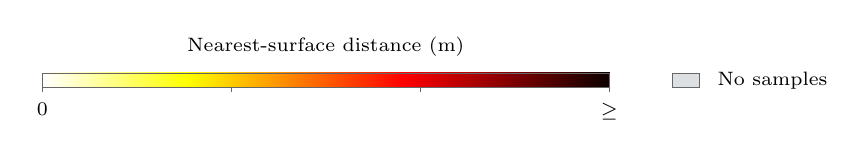
\begin{tikzpicture}[font=\scriptsize]
    \node[inner sep=0pt,anchor=south west] at (0,0) {\resizebox{7.2cm}{0.18cm}{\pgfuseshading{qualityerrorshading}}};
    \draw[black!60] (0,0) rectangle (7.2,0.18);
    \draw[black!60] (0,0) -- (0,-0.06);
    \node[anchor=north] at (0,-0.08) {0};
    \draw[black!60] (2.4,0) -- (2.4,-0.06);
    \node[anchor=north] at (2.4,-0.08) {\EvaluationQualityMapMiddleOne};
    \draw[black!60] (4.8,0) -- (4.8,-0.06);
    \node[anchor=north] at (4.8,-0.08) {\EvaluationQualityMapMiddleTwo};
    \draw[black!60] (7.2,0) -- (7.2,-0.06);
    \node[anchor=north] at (7.2,-0.08) {$\geq$\EvaluationQualityMapClip};
    \node[anchor=south] at (3.6,0.27) {Nearest-surface distance (m)};
    \filldraw[fill=qualitymapbackground,draw=black!60] (8.0,0) rectangle (8.35,0.18);
    \node[anchor=west] at (8.45,0.09) {No samples};
\end{tikzpicture}
